\documentclass[a4paper, 12pt]{book}
\usepackage[utf8x]{inputenc}   % omogoča uporabo slovenskih črk kodiranih v formatu UTF-8
\usepackage[slovene,english]{babel}    % naloži, med drugim, slovenske delilne vzorce
\usepackage[pdftex]{graphicx}  % omogoča vlaganje slik različnih formatov
\usepackage{fancyhdr}          % poskrbi, na primer, za glave strani
\usepackage{amssymb}           % dodatni simboli
\usepackage{amsmath}           % eqref, npr.
%\usepackage{hyperxmp}
\usepackage[hyphens]{url}  % dodal Solina
\usepackage{comment}       % dodal Solina

\usepackage[pdftex, colorlinks=true,
						citecolor=black, filecolor=black, 
						linkcolor=black, urlcolor=black,
						pagebackref=false, 
						pdfproducer={LaTeX}, pdfcreator={LaTeX}, hidelinks]{hyperref}

\usepackage{color}      
\usepackage{soul} 
\usepackage[numbers]{natbib}

\usepackage{listings} % For code showing

%%%%%%%%%%%%%%%%%%%%%%%%%%%%%%%%%%%%%%%%
%	DIPLOMA INFO
%%%%%%%%%%%%%%%%%%%%%%%%%%%%%%%%%%%%%%%%
% \newcommand{\fixspacing}{\vspace{0pt plus 1filll}\mbox{}}

\newcommand{\ttitle}{Različni pristopi umetne inteligence v video igrah}
\newcommand{\ttitleEn}{Different Artificial intelligence approaches in video games}
\newcommand{\tsubject}{\ttitle}
\newcommand{\tsubjectEn}{\ttitleEn}
\newcommand{\tauthor}{Jovan Prodanov}
\newcommand{\tkeywords}{računalniška igra, umetna inteligenca, računalnik, pristopi}
\newcommand{\tkeywordsEn}{computer game, artificial intelligence, computer, approaches}

\usepackage{hyperref}
%%%%%%%%%%%%%%%%%%%%%%%%%%%%%%%%%%%%%%%%
%	HYPERREF SETUP
%%%%%%%%%%%%%%%%%%%%%%%%%%%%%%%%%%%%%%%%
\hypersetup{pdftitle={\ttitle}}
\hypersetup{pdfsubject=\ttitleEn}
\hypersetup{pdfauthor={\tauthor, jp6957@student.uni-lj.si}}
\hypersetup{pdfkeywords=\tkeywordsEn}

%%%%%%%%%%%%%%%%%%%%%%%%%%%%%%%%%%%%%%%%
% PAGE SETUP
%%%%%%%%%%%%%%%%%%%%%%%%%%%%%%%%%%%%%%%% 
\addtolength{\marginparwidth}{-20pt} % robovi za tisk
\addtolength{\oddsidemargin}{40pt}
\addtolength{\evensidemargin}{-40pt}

\renewcommand{\baselinestretch}{1.3} % ustrezen razmik med vrsticami
\setlength{\headheight}{15pt}        % potreben prostor na vrhu
\renewcommand{\chaptermark}[1]
{\markboth{\MakeUppercase{\thechapter.\ #1}}{}} \renewcommand{\sectionmark}[1]
{\markright{\MakeUppercase{\thesection.\ #1}}} \renewcommand{\headrulewidth}{0.5pt} \renewcommand{\footrulewidth}{0pt}
\fancyhf{}
\fancyhead[LE,RO]{\sl \thepage} 
%\fancyhead[LO]{\sl \rightmark} \fancyhead[RE]{\sl \leftmark}
\fancyhead[RE]{\sc \tauthor}              % dodal Solina
\fancyhead[LO]{\sc Bachelor's thesis}     % dodal Solina

\newcommand{\BibTeX}{{\sc Bib}\TeX}

%%%%%%%%%%%%%%%%%%%%%%%%%%%%%%%%%%%%%%%%
% TITLES
%%%%%%%%%%%%%%%%%%%%%%%%%%%%%%%%%%%%%%%%  
\newcommand{\autfont}{\Large}
\newcommand{\titfont}{\LARGE\bf}
\newcommand{\clearemptydoublepage}{\newpage{\pagestyle{empty}\cleardoublepage}}
\setcounter{tocdepth}{1}	      % globina kazala

%%%%%%%%%%%%%%%%%%%%%%%%%%%%%%%%%%%%%%%%
% CONSTRUCTORS
%%%%%%%%%%%%%%%%%%%%%%%%%%%%%%%%%%%%%%%%  
% \newtheorem{izrek}{Izrek}[chapter]
% \newtheorem{trditev}{Trditev}[izrek]
% \newenvironment{dokaz}{\emph{Dokaz.}\ }{\hspace{\fill}{$\Box$}}

%%%%%%%%%%%%%%%%%%%%%%%%%%%%%%%%%%%%%%%%%%%%%%%%%%%%%%%%%%%%%%%%%%%%%%%%%%%%%%%
%% PDF-A
%%%%%%%%%%%%%%%%%%%%%%%%%%%%%%%%%%%%%%%%%%%%%%%%%%%%%%%%%%%%%%%%%%%%%%%%%%%%%%%

%%%%%%%%%%%%%%%%%%%%%%%%%%%%%%%%%%%%%%%% 
% define medatata
%%%%%%%%%%%%%%%%%%%%%%%%%%%%%%%%%%%%%%%% 
\def\Title{\ttitle}
\def\Author{\tauthor, ales.jaklic@fri.uni-lj.si}
\def\Subject{\ttitleEn}
\def\Keywords{\tkeywordsEn}

%%%%%%%%%%%%%%%%%%%%%%%%%%%%%%%%%%%%%%%% 
% \convertDate converts D:20080419103507+02'00' to 2008-04-19T10:35:07+02:00
%%%%%%%%%%%%%%%%%%%%%%%%%%%%%%%%%%%%%%%% 
\def\convertDate{%
    \getYear
}

{\catcode`\D=12
 \gdef\getYear D:#1#2#3#4{\edef\xYear{#1#2#3#4}\getMonth}
}
\def\getMonth#1#2{\edef\xMonth{#1#2}\getDay}
\def\getDay#1#2{\edef\xDay{#1#2}\getHour}
\def\getHour#1#2{\edef\xHour{#1#2}\getMin}
\def\getMin#1#2{\edef\xMin{#1#2}\getSec}
\def\getSec#1#2{\edef\xSec{#1#2}\getTZh}
\def\getTZh +#1#2{\edef\xTZh{#1#2}\getTZm}
\def\getTZm '#1#2'{%
    \edef\xTZm{#1#2}%
    \edef\convDate{\xYear-\xMonth-\xDay T\xHour:\xMin:\xSec+\xTZh:\xTZm}%
}

%\expandafter\convertDate\pdfcreationdate 

%%%%%%%%%%%%%%%%%%%%%%%%%%%%%%%%%%%%%%%%
% get pdftex version string
%%%%%%%%%%%%%%%%%%%%%%%%%%%%%%%%%%%%%%%% 
\newcount\countA
\countA=\pdftexversion
\advance \countA by -100
\def\pdftexVersionStr{pdfTeX-1.\the\countA.\pdftexrevision}


%%%%%%%%%%%%%%%%%%%%%%%%%%%%%%%%%%%%%%%%
% XMP data
%%%%%%%%%%%%%%%%%%%%%%%%%%%%%%%%%%%%%%%%  
\usepackage{xmpincl}
%\includexmp{pdfa-1b}

%%%%%%%%%%%%%%%%%%%%%%%%%%%%%%%%%%%%%%%%
% pdfInfo
%%%%%%%%%%%%%%%%%%%%%%%%%%%%%%%%%%%%%%%%  
\pdfinfo{%
    /Title    (\ttitle)
    /Author   (\tauthor, jp6957@student.uni-lj.si)
    /Subject  (\ttitleEn)
    /Keywords (\tkeywordsEn)
    /ModDate  (\pdfcreationdate)
    /Trapped  /False
}


%%%%%%%%%%%%%%%%%%%%%%%%%%%%%%%%%%%%%%%
% START
%%%%%%%%%%%%%%%%%%%%%%%%%%%%%%%%%%%%%%%
\begin{document}
\selectlanguage{english}
\frontmatter
\setcounter{page}{1} %
\renewcommand{\thepage}{}       % preprecimo težave s številkami strani v kazalu
\newcommand{\sn}[1]{"`#1"'}                    % dodal Solina (slovenski narekovaji)

%%%%%%%%%%%%%%%%%%%%%%%%%%%%%%%%%%%%%%%%
% INTRO
%%%%%%%%%%%%%%%%%%%%%%%%%%%%%%%%%%%%%%%%
 \thispagestyle{empty}%
   \begin{center}
    {\large\sc Univerza v Ljubljani\\%
      Fakulteta za računalništvo in informatiko}%
    \vskip 10em%
    {\autfont \tauthor\par}%
    {\titfont \ttitle \par}%
    {\vskip 2em \textsc{DIPLOMSKO DELO\\[2mm]
    VISOKOŠOLSKI STROKOVNI ŠTUDIJSKI PROGRAM PRVE STOPNJE RAČUNALNIŠTVO IN INFORMATIKA}\par}%
    \vfill\null%
    {\large \textsc{Mentor}: doc.\ dr.  Aleš Jaklič\par}%
    {\vskip 2em \large Ljubljana, 2022 \par}%
\end{center}

\clearemptydoublepage

%%%%%%%%%%%%%%%%%%%%%%%%%%%%%%%%%%%%%%%%
% INTRO ENGLISH
%%%%%%%%%%%%%%%%%%%%%%%%%%%%%%%%%%%%%%%%
 \thispagestyle{empty}%
   \begin{center}
    {\large\sc University of Ljubljana\\%
      Faculty of Computer and Information Science}%
    \vskip 10em%
    {\autfont \tauthor\par}%
    {\titfont \ttitleEn \par}%
    {\vskip 2em \textsc{Bachelor's Thesis\\[2mm]
    UNIVERSITY STUDY PROGRAMME UNDERGRADUATE PROGRAMMES COMPUTER AND INFORMATION SCIENCE}\par}%
    % Not sure if correct "University"
    \vfill\null%
    {\large \textsc{Mentor}: doc.\ dr.  Aleš Jaklič\par}%
    {\vskip 2em \large Ljubljana, 2022 \par}%
\end{center}


%%%%%%%%%%%%%%%%%%%%%%%%%%%%%%%%%%%%%%%%
% copyright page
%%%%%%%%%%%%%%%%%%%%%%%%%%%%%%%%%%%%%%%%
\thispagestyle{empty}
\vspace*{8cm}

\noindent
{\sc Copyright}. 
Rezultati diplomske naloge so intelektualna lastnina avtorja in matične fakultete Univerze v Ljubljani.
Za objavo in koriščenje rezultatov diplomske naloge je potrebno pisno privoljenje avtorja, fakultete ter mentorja.

\begin{center}
\mbox{}\vfill
\emph{Besedilo je oblikovano z urejevalnikom besedil \LaTeX.}
\end{center}
%%%%%%%%%%%%%%%%%%%%%%%%%%%%%%%%%%%%%%%%

\clearemptydoublepage

%%%%%%%%%%%%%%%%%%%%%%%%%%%%%%%%%%%%%%%%
% stran 3 med uvodnimi listi
\thispagestyle{empty}
\
\vfill

\bigskip
\noindent\textbf{Kandidat:} \tauthor\\
\noindent\textbf{Naslov:} \ttitle\\
\noindent\textbf{Vrsta naloge:} Diplomska naloga na visokošolskem programu prve stopnje Računalništvo in informatika \\
\noindent\textbf{Mentor:} doc. dr. Aleš Jaklič\\

\bigskip
\noindent\textbf{Opis:}\\

\bigskip
\noindent\textbf{Title:} \ttitleEn

\bigskip
\noindent\textbf{Description:}\\


\vfill

\vspace{2cm}

% prazna stran
\clearemptydoublepage

% zahvala
\thispagestyle{empty}\mbox{}\vfill\null\it%
\noindent
Zelo sem hvaležen vsem, ki so mi pomagali priti tja, kjer sem.
\rm\normalfont

% prazna stran
\clearemptydoublepage

%%%%%%%%%%%%%%%%%%%%%%%%%%%%%%%%%%%%%%%%
% posvetilo, če sama zahvala ne zadošča :-)
%%%%%%%%%%%%%%%%%%%%%%%%%%%%%%%%%%%%%%%%

\thispagestyle{empty}\mbox{}{\vskip0.20\textheight}\mbox{}\hfill\begin{minipage}{0.55\textwidth}%
Za svoja draga družina.
\normalfont\end{minipage}

% prazna stran
\clearemptydoublepage


%%%%%%%%%%%%%%%%%%%%%%%%%%%%%%%%%%%%%%%%
% kazalo
\pagestyle{empty}
\def\thepage{}% preprecimo tezave s stevilkami strani v kazalu
\tableofcontents{}


% prazna stran
\clearemptydoublepage


%%%%%%%%%%%%%%%%%%%%%%%%%%%%%%%%%%%%%%%%
% List of abbriviations
%%%%%%%%%%%%%%%%%%%%%%%%%%%%%%%%%%%%%%%%

% \chapter*{Seznam uporabljenih kratic}  % spremenil Solina, da predolge vrstice ne gredo preko desnega roba
\chapter*{List of abbreviations used}  % spremenil Solina, da predolge vrstice ne gredo preko desnega roba

\noindent\begin{tabular}{p{0.21\textwidth}|p{.4\textwidth}|p{.4\textwidth}}    % po potrebi razširi prvo kolono tabele na račun drugih dveh!
    % {\bf kratica} & {\bf angleško} & {\bf slovensko} \\ \hline
  {\bf Abbreviation} & {\bf English} & {\bf Slovenian} \\ \hline
  % after \\: \hline or \cline{col1-col2} \cline{col3-col4} ...
  {\bf ML}      & machine learning                  & strojno učenje \\
  {\bf FSM}     & finite state machine              & končni stroj \\
  {\bf NN}      & neural network                    & nevronska mreža \\
  {\bf NPC}     & non-player character              & neigralski lik \\
  {\bf BT }     & behaviour trees                   & drevesa vedenja \\
  {\bf RL }     & reinforcement learning            & učenje s krepitvijo \\
  \dots         & \dots                             & \dots \\
\end{tabular}

% prazna stran
\clearemptydoublepage

%%%%%%%%%%%%%%%%%%%%%%%%%%%%%%%%%%%%%%%%
% povzetek
%%%%%%%%%%%%%%%%%%%%%%%%%%%%%%%%%%%%%%%%

\addcontentsline{toc}{chapter}{Povzetek}
\chapter*{Povzetek}

\noindent\textbf{Naslov:} \ttitle
\bigskip

\noindent\textbf{Avtor:} \tauthor
\bigskip

%\noindent\textbf{Povzetek:} 
\noindent 
V diplomski nalogi bodo predstavljeni različni načini uporabe umetne inteligence v računalniških igrah s poudarkom na orodju, ki uporablja globoko okrepljeno učenje. Poglobili se bomo v zajčjo luknjo, ki je umetna inteligenca iger in poskušali razumeti leta raziskav. Celotne zgodovine umetne inteligence iger ne bi zajeli, vendar bo dovolj da ugotovimo kaj pomeni.
\bigskip

\noindent\textbf{Ključne besede:} \tkeywords.
% prazna stran
\clearemptydoublepage


%%%%%%%%%%%%%%%%%%%%%%%%%%%%%%%%%%%%%%%%
% abstract
%%%%%%%%%%%%%%%%%%%%%%%%%%%%%%%%%%%%%%%%

\selectlanguage{english}
\addcontentsline{toc}{chapter}{Abstract}
\chapter*{Abstract}

\noindent\textbf{Title:} \ttitleEn
\bigskip

\noindent\textbf{Author:} \tauthor
\bigskip

%\noindent\textbf{Abstract:} 
\noindent 
The thesis will present different ways of using artificial intelligence in computer games with an emphasis on a tool that uses deep reinforcement learning.
We will go deep into the rabbit hole that is game AI and try to understand years of research. The whole history of game AI will not be covered, but it will be enough to figure out what it means.
\bigskip



\noindent\textbf{Keywords:} \tkeywordsEn.
\selectlanguage{english}
% prazna stran
\clearemptydoublepage


%%%%%%%%%%%%%%%%%%%%%%%%%%%%%%%%%%%%%%%%
% START
%%%%%%%%%%%%%%%%%%%%%%%%%%%%%%%%%%%%%%%%

\mainmatter
\setcounter{page}{1}
\pagestyle{fancy}


\chapter{Introduction}

As soon as the first video game arrived, there was a need to create a more involved player experience. So, game developers created made characters or systems in their game to be controlled by game AI to let the player interact with the game on so many levels. Every year it passes that branch of game development is growing rapidly and hopefully soon to a new levels that we couldn't even think of.

But, creating an AI in video games comes with its own problems, in this thesis we will take our time to analyze and explain some techniques, and those techniques will be advancing in the order we are showcasing them. At the end we will conclude with possibly more knowledge of game AI than we have now and hopefully we can see a glimpse of the future of this topic that lies ahead.


\chapter{Background}
\label{ch1}
The question of game AI \cite{AIwiki} was present even in the first of games developed, by definition, in video games, AI is represented similar to human-like intelligence. The ways of approaching it are incredibly vast, in this thesis we will only scratch the surface, but focus on the most interesting ones.

\section{What is AI in games?}
First, I should start with the term "video game" \cite{VideoGameWiki}, it is a electronic game that involves a user interface and an input device (controller) to generate visual feedback. Then, the visual feedback is channeled to a displaying device, which can be observed. 

So, now for quite some time, game developers are trying to invent techniques and methods for incorporating intelligence into these video games. But, this AI is a broad term, in video games, it can mean: animation control, steering, flocking, pathfinding, planning, procedural generation, tactical and strategic thinking, learning \cite{FuzzyAIGames}, to name a few. Often, game AI can be mistaken for "true AI", which is to display human cognitive skills associated with human thinking, learning and problem-solving, but it most definitely is not.

Game AI adds another piece of the puzzle of defining AI and that is the illusion of intelligence. We would never want in a game an unbeatable ever-learning opponent, we would like a fun and easy experience, which isn't obviously stupid. Game AI in video games exists only to be fun and entertaining, so looking from this point, this is why the game developers are keen on sticking to things that are predictable and working and aren't experimenting a whole lot, because who would want unexpected things happening in a game.

\section{Illusion of intelligence}
Now that the secret is out, game developers were and are inventing tricks and techniques to make the player believe that games have real intelligence \cite{IllusionOfIntelligece}. And now, the main focus is the appearance of intelligence, rather than true intelligence.

\subsection{Why does it work?}
One of the reasons why this illusion works is that players want to believe that there are glimmers of real human-like intelligence in their virtual worlds \cite{IllusionOfIntelligece}. Also, the players are easily forgiving with their high expectations.

Another reason why it works is because of anthropomorphism \cite{AnthropomorphicCharacters}, which is the interpolations of human behaviours to inanimate objects, this can be related to animated characters in video games. There is a research that preschool kids were 91\% likely to pick a character that is not a human being.

As previously stated, expectations have a high influence. Because of the placebo effect, if players are expecting a highly intelligent game, their enjoyment will be higher. This is the same as if people think they are eating a more expensive food or a drink, they are more likely to enjoy it.

\subsection{Selling it}
The illusion of intelligence \cite{IllusionOfIntelligece} works when there is a certain level of quality to it, and that quality is helped by:
\begin{itemize}
    \item \emph{Animation and dialog} - this helps with the interaction with the world and player, as well as making the experience more alive and present.
    \item Although animations help to achieve game AI, it should be done with quality. They should the smooth and human-like, instead of looking like a - \emph{robot}.
    \item \emph{Have a reason to exist} - AI characters shouldn't always wait for the player to approach, they should have their own purpose. As well as their own motives, because the game world would be their home and reality and they should have their own states in it.
    \item The culmination of building a successful AI character would be for it to have its own - \emph{personality}. How the game developer leverages this powerful tool can complete change the feel of the game.
\end{itemize}


\section{Deterministic vs Non-deterministic}
It is in close connection to game AI that there exists two type of games. In a deterministic game, the course of the game depends only on the players’ decisions, but in a non-deterministic game, there’s some factor of randomness involved \cite{DeepLearningGO}. % ?

For example, chess is a deterministic game, the outcome of the game is entirely based on the players' decisions. But, football is non-deterministic, the players can't reliably kick the ball exactly the same every time. In that sense, luck or randomness often makes the game more exciting, however too much randomness removes all influence of the player in game, which is rarely fun.


\chapter{Current AI in games}
\label{ch2}

So, advanced techniques for game AI have been spotted more often, for examples, there have been usages of Bayesian networks and neural networks for real-time strategy games, as well as evolutionary algorithms. But, in those cases the game seems to orbit around that as the main focus of the game itself. In other words, advanced techniques for game AI currently need a game to be build around them. Then, there is the problem of these techniques needing a high computational and memory power. Also, the last problem would be their non-determinism, that just brings more problems to the table and game developers are reluctant to ship a game that is not tested enough.

In this chapter, we will focus more on the current techniques that are widely used, which finely sell the illusion of intelligence.

\section{Finite State Machines}

You want to create a side-scrolling platformer, the first thing to do is make a plan. We start off by drawing a box for everything the main character can do: stand, jump, duck, shoot. When the players gives some kind of input, for an example a button is pressed, there is an arrow from  that box with the name of the button labeled and connected to the other box that it changes to.

\begin{figure}[h]
\begin{center}
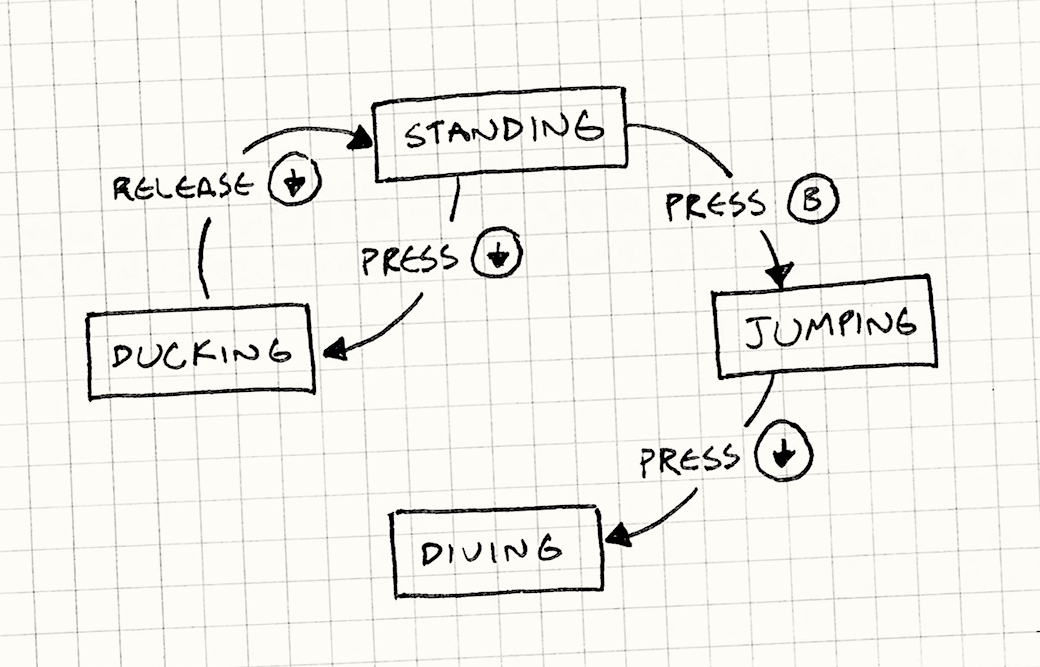
\includegraphics[width=0.5\textwidth]{Images/state_FSM.png}
\end{center}
\caption{Finite State Machine}
\label{pic1}
\end{figure}

Congratulations, we have successfully created a FSM \cite{GameProgrammingPattersFMS}. The idea of it came out of a computer science branch called \emph{automata theory}, which includes the famous Turing machine \cite{TuringMachine}. It should be noted that FSMs are the simplest of that bunch. The rules are simple:
\begin{itemize}
    \item The number of states is fixed.
    \item The current state can be only one.
    \item Inputs or events can be sent to the machine.
    \item Each state has a set of transitions, each associated with an input/event and pointing to a state
\end{itemize}

So, now that I've introduced FSMs, there is a catch. 
The reason why state machines work to untangle complicated code is because they force a constrained structure on it - they force a numbered set of states, only one current state and hard coded transitions. However, when wanting to create a more complex game AI, you have to work around these problems, we'll dive deeper into them. 

\subsection{Concurrent State Machines}

Let's now equip our hero with a gun. If we want to play by the constraints of an FSM, we have to double our states: standing, standing with a gun, jumping, jumping with a gun etc. Its redundant, however we can add another state into a single machine, what the hero is doing and what he's carrying.

\begin{verbatim}
class Hero  {
    private State _state;
    private State _equipment;

    private void HandleInput(Input input) {
        _state.HandleInput(input);
        _equipment.HandleInput(input);
    }
}
\end{verbatim}

\subsection{Hierarchical State Machines}

So, when we don't want to repeat our code in all of our states, we can define one state that handles multiple other states. E.g. we can create a \texttt{OnGround} state that can handle walking, and other states like running can inherit from walking and add it to its behaviour.


This is called \emph{hierarchical state machine} - states can have super-states, that means that if an input/event comes and the current (sub-state) can't handle it, it gets transferred to the chain of super-states. It can be understood like overriding inherited methods.

To clarify, if an input/event starts at a sub-state, it gets passed up the ladder until one handles it - if none do, it is ignored.

\subsection{Pushdown Automata}

This is an extension to FSMs, that uses the concept of stacks. The problem is with basic FSMs is that you don't have history of the previous states. You know of what state you \emph{are} currently in, but no memory of what state you \emph{were}.

In FSMs, only a pointer to the current state exists, pushdown automata has a stack of pointers. In a FSM, transitioning into the new state just replaces the previous pointer. Pushdown automata let's you choose:
\begin{itemize}
    \item Push a new state on the stack, this transitions to it, but it leaves the previous state directly under instead of discarding.
    \item Pop the current state, in doing so, the state that is under it becomes the new current state.
\end{itemize}

\begin{figure}[h]
\begin{center}
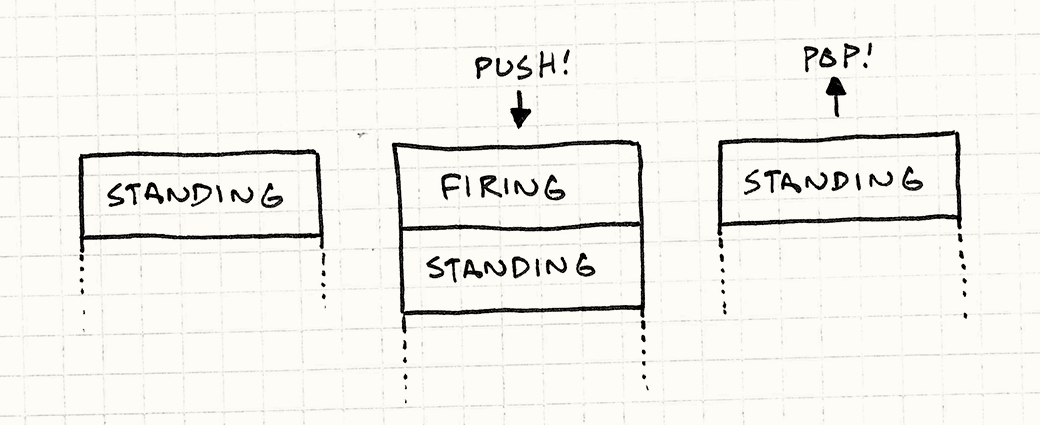
\includegraphics[width=0.6\textwidth]{Images/state_pushdown.png}
\end{center}
\caption{The Pushdown Automata}
\label{pic2}
\end{figure}

\subsection{Example}

Best way to present FSMs is to start with a simple, but upgradable example for future extensibility. For this example, I will use the sprites from a game that I created \cite{KWA}, in the figure \ref{KWA}. It will have a basic state machine with states for: \emph{idle} (grounded), \emph{moving} and \emph{jumping} in the figure \ref{StateMachine}.

\begin{figure}[!hb]
\minipage{0.32\textwidth}
  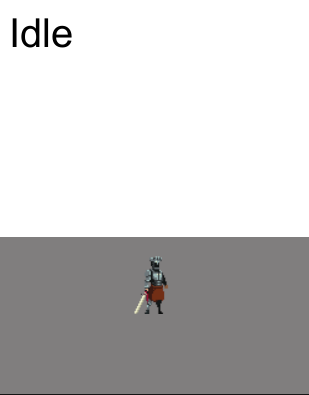
\includegraphics[width=\linewidth]{Images/IdleState.png}
  \caption{Idle}\label{StateFig:Idle}
\endminipage\hfill
\minipage{0.32\textwidth}
  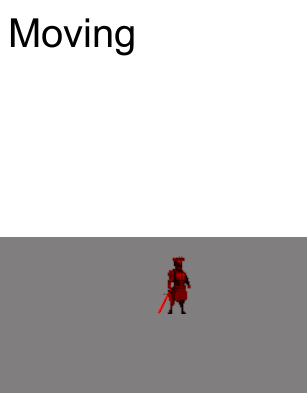
\includegraphics[width=\linewidth]{Images/MovingState.png}
  \caption{Moving}\label{StateFig:Moving}
\endminipage\hfill
\minipage{0.32\textwidth}%
  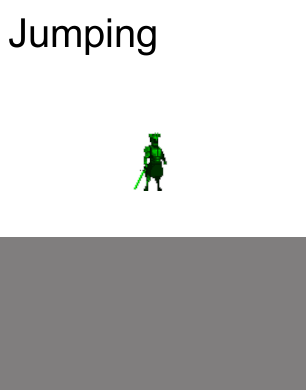
\includegraphics[width=\linewidth]{Images/JumpingState.png}
  \caption{Jumping}\label{StateFig:Jumping}
\endminipage
\label{StateMachine}
\end{figure}

The \texttt{StateMachine} is meant to be overwritten with our movement script. It has a attribute of \texttt{BaseState} and with methods: 
\begin{itemize}
    \item \texttt{Start()} - Sets the current state to the initial state and if there is an initial states, it enters it.
    \item \texttt{Update()} - If there is a current states, it updates the logic in it.
    \item \texttt{LateUpdate()} - If there is a current states, it updates the physics in it.
    \item \texttt{ChangeState(BaseState newState)} - Exists the current state, sets it to the new state and enters the new state.
    \item \texttt{GetInitialState()} - This is a virtual method so we need to override it in our script.
    \item \emph{Misc} - GUI method which displays the current state.
\end{itemize}

The \texttt{BaseState} script serves for all the states our machine can have. It has attributes like a name and a state machine which it reads from. Also, it has virtual methods meant to be overwritten: \texttt{Enter()}, \texttt{UpdateLogic()}, \texttt{UpdatePhysics()} and \texttt{Exit()}.

And thats nearly it, we have set the basis of our state machine, now we just have to implement it for our movement. We create a movement state machine with 3 states: \texttt{IdleState} (which is set to be the initial state), \texttt{MovingState}, \texttt{JumpingState}. We have the basic logic for movement in those states and we just color our sprite every time it enters the said state.

\clearpage

\section{Behaviour Trees}

Even with extensions to FSMs, they are pretty limited. If the aim is complex game AI, the previous chapter only whet our appetite.

Behaviour trees (BTs) \cite{BehaviourTreeStarterPack} are proven to be a extensive technique which can create a pretty versatile AI. It makes a solid foundation for combining other techniques and to have full control over behaviour and performance.

So, to define a BT, it is an structure that is made up from nodes which have separate behaviours - individual actions which can be performed. In turn, each node has its own child behaviours, which gives the algorithms its tree-shaped structure. In addition, each behaviour has its own condition which lets the algorithm pass to the child branches.

\begin{figure}[h]
\begin{center}
    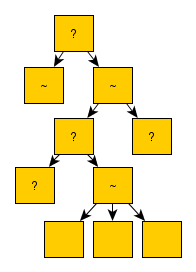
\includegraphics[width=0.35\textwidth]{Images/behaviour_tree.png}
\end{center}
\caption{Behavior Tree}
\label{pic3}
\end{figure}

Every behaviour has its own condition and an action. The algorithm starts at the root of the tree and at each levels examines the conditions of the behaviours. If a condition matches of a node, it executes the action. None of its siblings will be examined, but its children will. The algorithm is as it follows:
\begin{verbatim}
    Make root node the current node
    While current node exists
        Run current node's condition
        If condition returns true
            Add node to execute list
            Make node's child current node
        Else
            Make node's sibling current node
    Run all behaviors on the execute list
\end{verbatim}

The strength of BTs \cite{BehaviourSelectionAlgorithms} is their simplicity. Since trees have no states, the algorithm doesn't have to remember what behaviours were running and behaviours can be written without them being aware of each other. Extensibility is also a big plus, it is very easy to add more functionability at any given time.

But and now this is a big but, although BT algorithm is simple and powerful, its not always the best choice. The algorithm has to start at the root node every time a new behaviour is chosen, that means the running time is greatly impacted, in comparison to FSMs. Also, it deals with a lot of conditionals. Furthermore, memory is a problem as behaviours can loop with each other, however steps can be taken to deal with this problem.

\section{Scripting, the good and the bad}

Now we're about to talk the most controversial game AI that has ever been created. From it, it can come out to be the best game AI to ever be... or some of the worst. It all depends on its implementation.

However, to have a successful scripted AI, one must not fear it. Like any weapon, the soldier must first learn how to use to and master it through trial and error. 
The game's architecture can handle scripting techniques a couple of ways - for the most part, they use the two ideologies \emph{master and servant} \cite{ForbiddenScripting}. While both have their purpose, it is useful to acknowledge which role the scripted AI will play in the game's development.

\subsection{Master and Servant ideology}

To start off, to be successful into making a scripted AI, it is important to understand how much the AI depends on the overall foundation of the said game. The game systems and architecture must be thoroughly thought out to have an effective scripted AI. Without it, the AI can produce huge amount of bugs, or even halt/stop development.

So the most viable technique for scripted AI would be the master and servant approach. In short, the master script would take care of the high-level aspects of the game, while the servant script would control the overall activity of the agents, or just create some kind of effects.  

\begin{itemize}
    \item \emph{Master scripts} work best in two scenarios. The first one would be if in game already exists some kind of AI, and the scripting would be the glue that combines this techniques into a powerful model for agent behaviour. Even in the other scenario when its only the scripting technique, it can produce good results for different decision-making and planning techniques.
    \item \emph{Servant scripts} are best effective when design requires a high degree in specificity in agent behaviour. So special case scenarios are created by the developers for each agent and this can have excellent results for ambient or background AI.
\end{itemize}

Games, would often tip themselves into one side or the other. It it dependant to a lot of circumstances: the experience of the developers, time and budget, the ratio of programmers to designers etc.

There is a stigma justified by negativity of players not enjoying games with scripted AI, which show little depth or variety to their AI. But, with proper coordination between design and technical concerns of the project, scripted AI could become a powerful tool with a lot of depth and players would be grateful.

Moreover, scripting should be used in combination with other techniques, due to over-reliance on scripts is why we get the shallow and unwanted AI. On an another page, developers must resist the urge to anticipate everything that a script might need to handle. This can be avoided with delegation, but the most important is having a chosen design early on and sticking to it, whether be it master and servant approach. When it comes to scripting, often simpler is better, instead of having to design overly complicated and intricate systems, its better to stick on more flexible and creative solutions.

\subsection{Example}

For scripted AI, there is a perfect example - a game that I made not so long ago using the MonoGame framework. % I Should cite it
The game \cite{KWA} consists of a knight roaming with his dog, but the dog gets scared of some skeletons and now the knight has to defeat skeletons in order to chase and recover his dog, we can see it in figure \ref{KWA}.

\begin{figure}[h]
\begin{center}
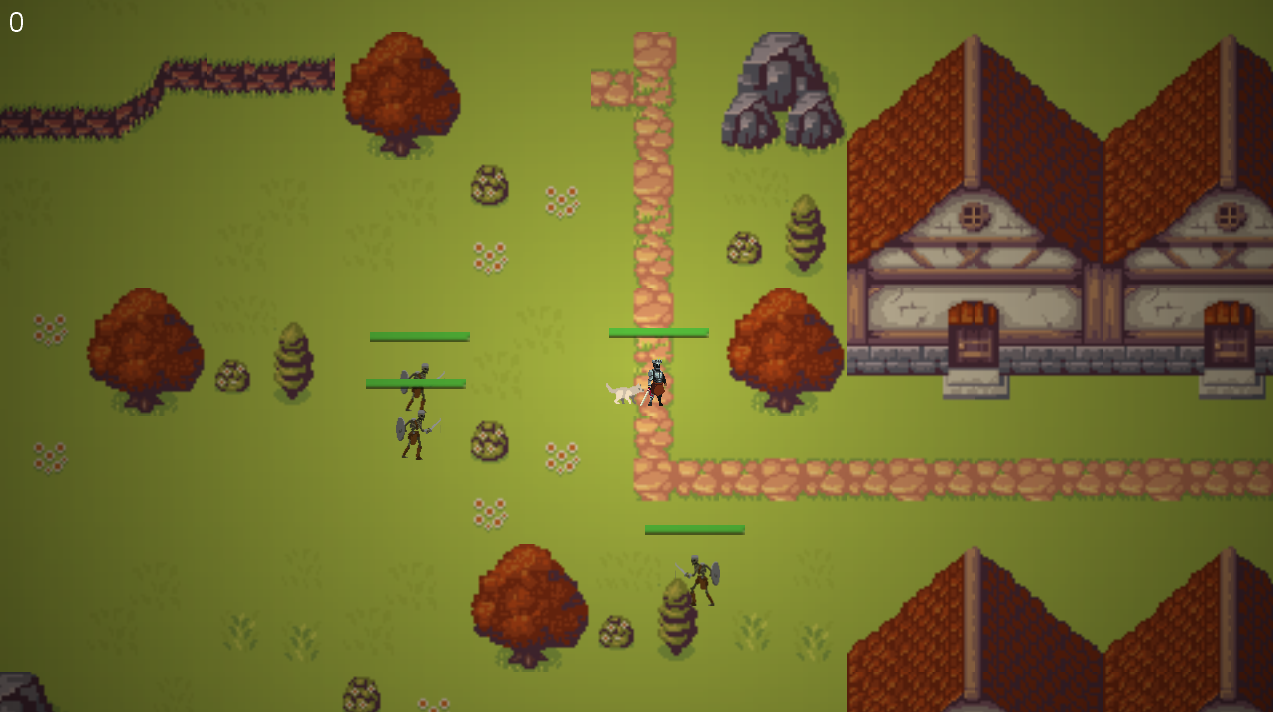
\includegraphics[width=0.5\textwidth]{Images/KWAtown.png}
\end{center}
\caption{Picture of the game with the skeleton enemies}
\label{KWA}
\end{figure}

From this game, I wanted to present the skeleton AI, because is the perfect example for scripted AI. Down below is a mimic of the code, but the functionality is the same. The skeleton has some private attributes that he uses with his scripted AI.


\lstinputlisting[language={[Sharp]C}, basicstyle=\small]{Code/KWADemo.cs}

This can be an example of the servant scripted AI, because there is a lot of skeletons spawned and this script is used on each one of them. The code basically executes only for the lifespan of the skeleton, and while alive, it checks if the player attacks him and tries to go towards him if it has seen him. If the skeleton is close enough, it will attack.

\section{Fuzzy Logic}

Fuzzy logic \cite{FuzzyAIGames} is a super set of conventional logic that has been extended to handle the concept of partial-truth values between the boolean dichotomy of true and false. It usually has its own components like fuzzy variables, fuzzy rules and fuzzy interface engines.

As well as the previous techniques, fuzzy logic has the goal of a simple design resulting in intelligent agents. Controlling a game character with fuzzy logic can be done easily due to suitable input and output values.

Fuzzy logic is an extension of \emph{crisp logic} (conventional logic), there is the same as binary logic, the variable can be true or false. In crisp logic, the variables can be from a set of two elements, while in fuzzy logic \cite{FuzzyLogicBasedGameSystem}, the concept has been extended to handle partial-truth values between true and false. 

For example, the weapon range can be divided into melee, ranged or out of range as seen in \ref{pic4}.

\begin{figure}[h]
\begin{center}
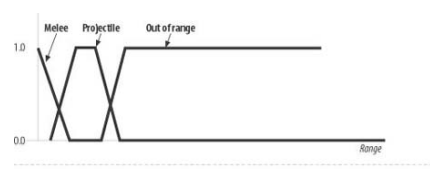
\includegraphics[width=0.53\textwidth]{Images/weapon_range.png}
\end{center}
\caption{Weapon range with Fuzzy Logic}
\label{pic4}
\end{figure}

Fuzzy logic brings a lot to the table when it come to game AI. It can help in NPC decision making or even weapon selection. With its benefits it can lead to an advanced AI with a pretty simple implementation. It can be even used in combination with FSMs (when transitioning from one state to another) and BTs (when branching out). For example, with conventional logic a car can only brake and accelerate, but with fuzzy logic it can be stated how much should the car brake and accelerate due to the gradual behaviour. 

\subsection{Pitfalls}

As good as fuzzy logic sounds till now, I have to talk about its downsides. Due to its knowledge-based nature, it requires a correct definition of input and output variables, as well as their relationships. Another downside, if the system of fuzzy logic is not designed carefully, it can lead to a lot of rules being checked at a given moment and sacrificing its advantage of a low computational cost.

In a video game, there can be many input variables to an agent's behaviour, each with their own number fuzzy sets. Because of this, the fuzzy rules can grow exponentially and it could even lead to combinatorial explosion \cite{CombinatorialBombing}.

\section{Flocking}

Flocking is a technique used to simulate intelligent movement of groups, the groups are called \emph{boids}. It is mostly used when NPCs need to move in a cohesive unit rather then independently. The genre of games that use this technique the most is RTS (Real-time strategy) games. The name "flocking" comes from flock of birds.

The one who's responsible for the flocking algorithm is Craig W Reynolds with his groundbreaking research \cite{FlocksReynolds}. His implementation is leaderless, is made in way that no boid leads the flock, they all just follow the group - which seems to have a mind of its own.

The flocking behaviour can be simulated by using three principles \cite{FlockingBehaviour}: 
\begin{itemize}
    \item \emph{Alignment} - Keeps track of the average velocities and keeps check of the boids' velocities and tries to keep the average speed.
    \item \emph{Cohesion} - Computes the direction of the average position of the boids and tries to steer all the boids for them to be together as a group.
    \item \emph{Separation} - Each boid knows the distances of its neighbors, so with that knowledge it tries to apply an repulsive force in the opposite direction to maintain distance from them. In a way, it is a collision avoidance within the flock.
\end{itemize}

\begin{figure}[!htb]
\minipage{0.32\textwidth}
  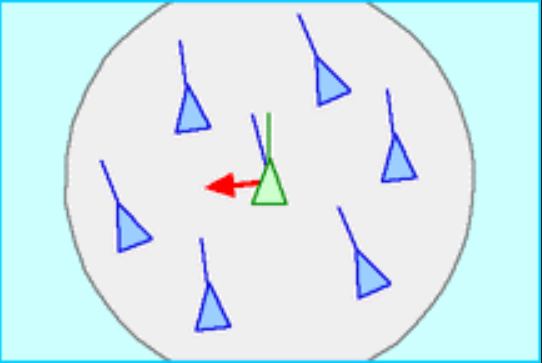
\includegraphics[width=\linewidth]{Images/alignment.png}
  \caption{Alignment}\label{fig:image3}
\endminipage\hfill
\minipage{0.32\textwidth}
  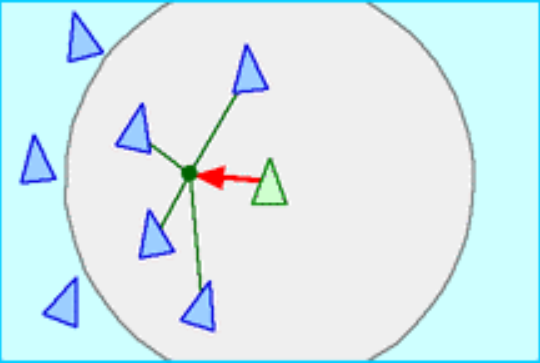
\includegraphics[width=\linewidth]{Images/cohesion.png}
  \caption{Cohesion}\label{fig:image2}
\endminipage\hfill
\minipage{0.32\textwidth}%
  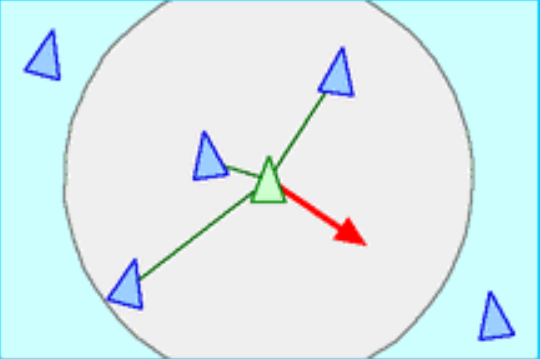
\includegraphics[width=\linewidth]{Images/separation.png}
  \caption{Separation}\label{fig:image1}
\endminipage
\label{pic5}
\end{figure}

The path of the boids which want to move is calculated by the A* pathfinding algorithm \cite{FOEAD2021507}. Its simple purpose is to find the shortest path from point A to point B. Its a well known method to use as a basis for pathfinding problems with its known  simplicty, efficency and modularity.

But, A* algorithm isn't fool proof, in many cases it would need a supplementary algorithm or a tweak to its core mechanics. Also, A* may find a path much quicker than other searches, but it does not ensure that the result will be the shortest path. Research shows that A* will have a correct result only 85\% of the time \cite{FOEAD2021507}. Overall, the traditional algorithm can't keep with the modern requirements of pathfinding, so game developers are needed to tweak and enforce it for adequate results.

\clearpage

\subsection{Example}

So the example works in a way that it calculates separation, cohesion, alignment in every \texttt{Update()} call. So, that means its a pretty expensive, but for a demonstration, it will do just fine. Most of the time it a has a time complexity of $ \mathcal{O}(n^2) $.

\begin{figure}[h]
\begin{center}
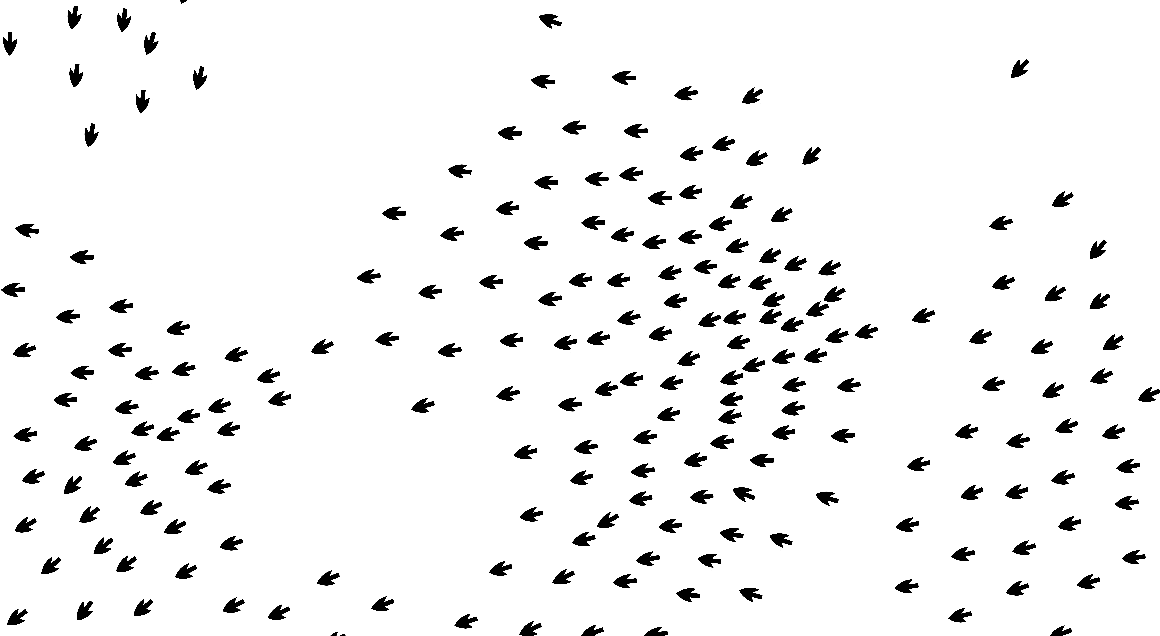
\includegraphics[width=0.6\textwidth]{Images/FlockingExample.png}
\end{center}
\caption{Flocking example with 200 boids}
\label{100boids}
\end{figure}

We can start with 200 boids at first in figure \ref{100boids}, we can see that right away they formed two flocks, but later on disperse. So, we have three methods for calculating alignment, cohesion, separation amount, the rules for the algorithm them are:
\begin{itemize}
    \item \emph{Alignment} - The boids face the same direction.

\lstdefinestyle{sharpc}{language=[Sharp]C, basicstyle=\small}
\lstset{style=sharpc}
% Alignment code ------
\begin{lstlisting}
var velocity = Vector2.zero;
foreach (var boid in boids)
{
    velocity += boid.velocity;
}
velocity /= boids.Count();
var steer = (velocity.normalized * maxSpeed) - velocity;
return steer;
\end{lstlisting}
% Alignment code ------

    The vector is calculated using neighboring units' normalized velocity vector.
    \item \emph{Cohesion} - The boids move to the center of mass of its neighbours.

% Cohesion code ---------
\begin{lstlisting}
var sumPositions = Vector2.zero;
foreach (var boid in boids)
{
    sumPositions += boid.Position;
}
var average = sumPositions / boids.Count();
var direction = average - Position;
var steer = (velocity.normalized * maxSpeed) - velocity;
return steer;
\end{lstlisting}
% Cohesion code ---------

    The vector is calculated using the difference between the neighbor's position and the unit's position.
    \item \emph{Separation} - The boids attempt to move away from the neighbours who are too close.

% Separation code ---------
\begin{lstlisting}
var direction = Vector2.zero;
boids = boids.Where(DistanceTo(o) <= neighborhoodRadius / 2);
foreach (var boid in boids)
{
    var difference = Position - boid.Position;
    direction += difference.normalized / difference.magnitude;
}
direction /= boids.Count();
var steer = (velocity.normalized * maxSpeed) - velocity;
return steer;
\end{lstlisting}
% Separation code ---------

    The vector is the opposite of the cohesion vector.
\end{itemize}

Then, we get the final acceleration which is calculated as the weighted sum of the results of these three methods \texttt{alignmentSteer * alignment + cohesionSteer * cohesion + separationSteer * separation}.

While this example for flocking \cite{FlocksReynolds} has focused on movements that are similar to fish or herd of birds, the algorithm can be extended to express movement of other animals. The realism can be furthered by tweaking the parameters of the algorithm.

\section{Genetics Algorithm}

A genetic algorithm \cite{GameAIGeneticAlg} is a probabilistic algorithm that generates an approximate solution based on Darwin’s Theory of Evolution. The basic gist of the algorithm is producing new off-springs from an existing population and then selecting the fittest off-springs from that populating for the next generations. This algorithm has been around for several decades so there may exist a lot of variations.

In this section, we'll take a look into a certain genetic algorithm, which we need to define some terms for:

\begin{itemize}
    \item \emph{Gene} - Single parameter of search space
    \item \emph{Chromosome} - Collection of genes
    \item \emph{Individual} - Instantiated chromosome
    \item \emph{Population} - Collection of individuals
    \item \emph{Fitness} - Evaluation of an individual in our selected problem
    \item \emph{Crossover} - Process to create a new individual by breeding two
    \item \emph{Mutation} - Process to randomly change some genes to oppose local optima (solution that is optimal within a neighboring set of candidate solutions \cite{LocalOptimum}) 
    \item \emph{Generation} - One iteration of the Genetics Algorithm
\end{itemize}

Now, that we have defined some general terms we need for the algorithm, we can go ahead and get into it:

\begin{verbatim}
    Generate an initial random population
    Calculate fitness of every individual of the population
    Copy the individual over to the next generation
    Randomly mutate certain genes of individuals in the current generation
    From the mutated generation, choose pairs of individuals of certain 
        fitness to crossover
    If the number of maximum iterations of generation is not reached, 
        go the second line
\end{verbatim}

The best for a probabilistic algorithm is to iterate until there is no improvements, but in the genetic algorithm we need to set up a number of iterations, because it always mutates.

The usage of genetics algorithms is immense, it can robustly and effectively search a poorly search space, when we have scarce knowledge. It is best for non-linear problems. The appeal of this algorithm comes from its elegance and simplicity for its power to discover good solutions for high-dimensional problems \cite{CurrentAIGames}.

And for the downsides, genetics algorithms require high computational and memory power, so it has big drawback when playing a game with it. Game developers mainly manage this by executing the algorithm when the game is not being played. In summary, its an effective algorithm based on evolution and natural selection and its used for learning and optimization.

\chapter{ML-Agents}
\label{ch3}

\section{Technologies}

To correctly use the ML-Agents toolkit we would need certain type of technologies. If we want to use the ML-Agents toolkit with Unity, we start with the Unity editor and Unity game engine \cite{UnitySoftware}. In the Unity editor, in the Package Manager, we should install "ML Agents".

After, we should have (or install) Python \cite{PythonManual} (I used python 3.9). With python pip we would need the packages pytorch (\texttt{torch}) and \texttt{mlagents} - For this step I chose to have a virtual environment, which is beneficial to have the proper versions and have the setting up part more organized.

Now, we are good to go, with the command \texttt{mlagents-learn} and Unity open we could freely proceed into the chapter with ease.

\section{Background}

After we've checked out some the key game AI that are used in the industry, I would like to present an open-source project The Unity Machine Learning Agents Toolkit or ML-Agents Toolkit. It is used for training intelligent agents through reinforcement learning, imitation learning, neuroevolution, or other ML methods through a simple-to-use Python API \cite{MLAgents}.

\subsection{Agents}

The technology of ML-Agents is mostly used for training Agents, which are basically NPCs, we can use variety of methods for the training. But, first we need to explain three entities of the game, which is the environment of the training.

\begin{itemize}
    \item \emph{Observations} - How the Agent sees the environment, the observations can be numeric and/or visual. Numeric observations can be some kind of attributes taken from the environment (they can be discrete or continuous), for the best results, the agent should have several continuous numerical observations. Visual observations are images generated from the cameras that are attached to our agent. The observations are separate from the environment, so that so that the agent can't get confused with data coming from the whole game/environment.
    \item \emph{Actions} - What can the agent do, same as the observations, the actions can be discrete or continuous. They can get as complex as the environment allows them to be.
    \item \emph{Reward signals} - How well the agent is doing, these signals don't have to be sent at every moment. The agent should be rewarded only when he does some action that is good, and punished when it does something bad. It should be noted that the rewarding is how the objective of the agent is communicated, so it should be set up in an optimal way for best results.
\end{itemize}

\subsection{Architecture}

The ML-Agents toolkit system works with 5 connected high-level components. And those are:

\begin{itemize}
    \item \emph{Learning environment} - is actually the Unity scene and all the game objects. This scene is used either for training or for testing environments, this is where the above aforementioned Unity package ML Agents comes in handy. With it, the agents and their behaviours get defined.
    \item \emph{Python low-level API} - is interacting and manipulating the learning environment, it lives outside of the learning environment and interacts with it through the External communicator.
    \item \emph{External communicator} - connect the learning environment with the python low-level API, it actually lives in the learning environment.
    \item \emph{Python trainers} - contains all the ML algorithms, they are all contained in the python \texttt{mlagents} package.
    \item \emph{Gym wrapper} - common way in which ML researchers interact with learning environments is with the wrapper from openAI called gym \cite{openAIGym}.
\end{itemize}

\begin{figure}[h]
\begin{center}
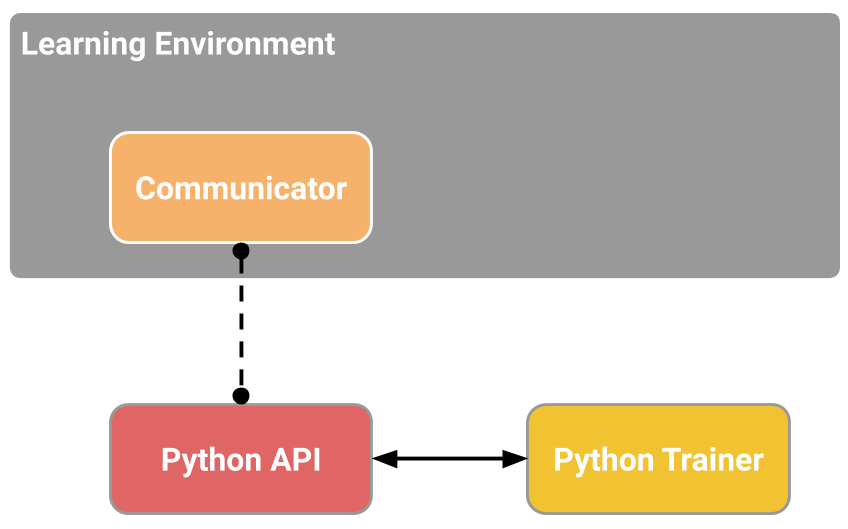
\includegraphics[width=0.7\textwidth]{Images/learning_environment_basic.png}
\end{center}
\caption{Simplified ML-Agents architecture \cite{MLAgents}}
\label{pic6}
\end{figure}


\clearpage

The learning environment in the Unity scene has two components:
\begin{itemize}
    \item \emph{Agent} - is linked to Game Object, handles the observations, actions and rewards.
    \item \emph{Behavior} - defines the attributes and number of actions the agent can take. It can be described as a function that takes the observations and rewards from the agent class and returns the actions. The behaviour can be one of three types:
    \begin{itemize}
        \item \emph{Learning} - not defined, about to be trained.
        \item \emph{Heuristic} - its defined by hard-coded rules, mainly is used for input for controlling the agent.
        \item \emph{Inference} - is already trained, and contains a already working and trained Neural Network file.
    \end{itemize}
    Basically, after a learning behaviour is trained, it becomes an inference behaviour.
\end{itemize}

With that knowledge of the architecture of ML-Agents, we can present how a game would look.

\begin{figure}[h]
\begin{center}
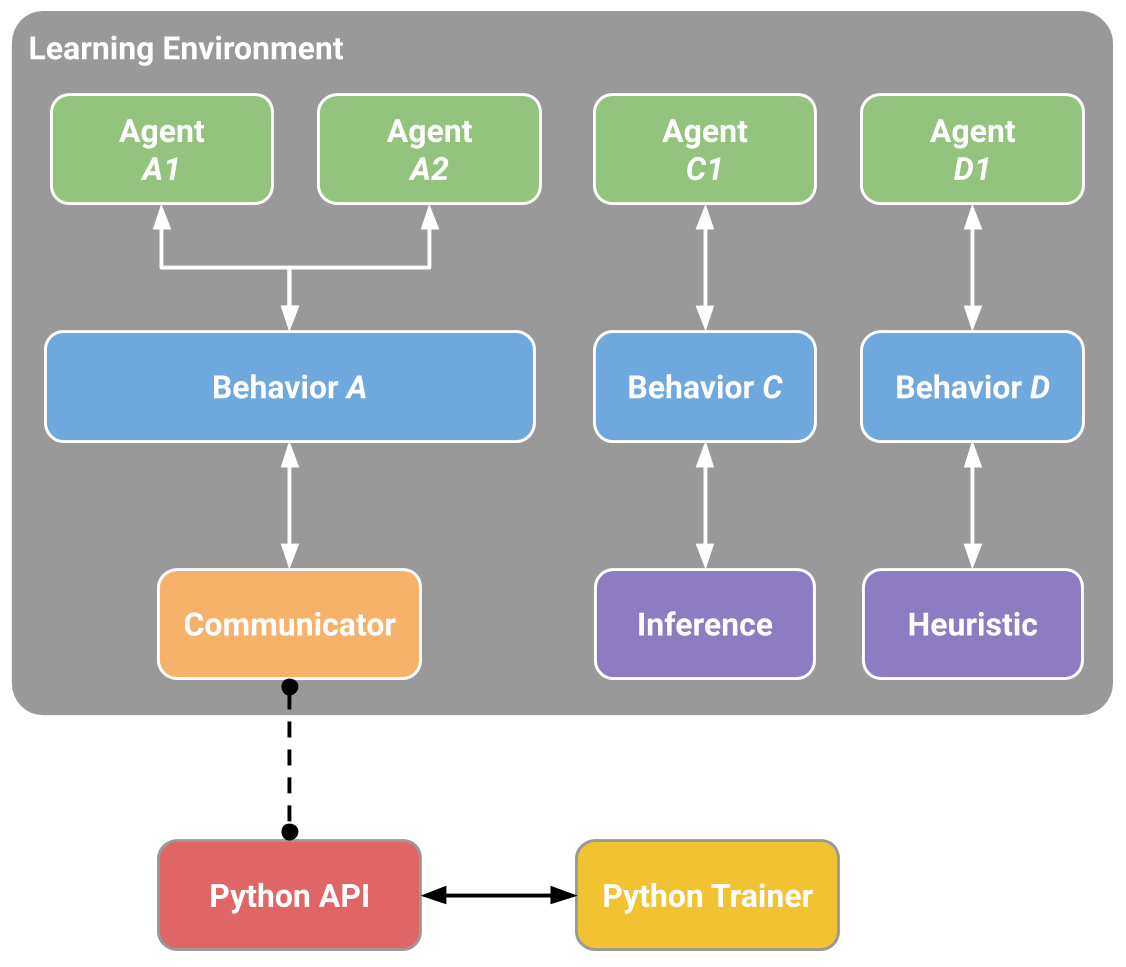
\includegraphics[width=0.5\textwidth]{Images/learning_environment_example.png}
\end{center}
\caption{Example of how the architecture looks of a simple game}
\label{pic7}
\end{figure}

\subsection{Training methods}

Before I jump into the examples, I would like a to showcase a brief overview of the ML algorithms that are a part of ML-Agents.

\subsubsection{Note on rewards signals}

A quick note is that rewards in ML-Agents can be \emph{intrinsic} or \emph{extrinsic}. Rewards that the agent can get from the learning environment are called extrinsic. But, rewards can be also defined outside of the envirnonment, we refer these as intrinsic rewards.

With the toolkit, the reward signals can be tweaked in four ways:
\begin{itemize}
    \item \texttt{extrinsic} - represents the rewards in the environment, its on by default
    \item \texttt{gail} - represents the intrinsic rewards defined by GAIL (we will take a look at it down below)
    \item \texttt{curiosity} - represents the intrinsic reward that encourages the player to explore, it is defined by a Curiosity module
    \item \texttt{rnd} - represents the intrinsic reward that encourages the player to explore, it is defined by a Curiosity module
\end{itemize}

\subsubsection{Deep reinforcement learning}

ML-Agents has implementation of two algorithms Proximal Policy Optimization (PPO) and Soft Actor-Critic (SAC). The default is PPO as it has been proven to be more general purpose and more stable. On the other had SAC, tends to collect sets of experiences and learn from them. So when looking from an efficiency point of view, PPO would require more samples, so from that SAC is the better choice for heavier environments. Also, SAC encourages exploration, as it is an "maximum entropy" algorithm.

The curiosity reward signal, which we mentioned earlier, is managed by the Intrinsic Curiosity Module. Its an implementation in ML-Agents inspired by "Curiosity-driven Exploration by Self-supervised Prediction" \cite{CuriosityExploration}. When we are at this topic, RND, which is \emph{Random Network Distillation} \cite{ExplorationRND} is also a module in ML-Agents that helps out with the agent's exploration.

\subsubsection{Imitation Learning}

Often when training, the agents can have a hard time at the beginning of the training. So, in order to prevent or help that process, it can be demonstrated the wanted behaviour to the agent and it can learn from that, rather than trying and trying. This is called \emph{imitation learning}, even better it can even be combined in conjunction with the already existing reinforcement learning. In doing that, the time for the agent to learn the behaviour drops down drastically.

For the imitation learning, ML-Agents uses two algorithms called Behavioral Cloning (BC) and Generative Adversarial Imitation Learning (GAIL). In order to make the agents learn through demonstrations, GAIL and BC have to be enabled in the proper \texttt{yaml} configuration file.

The demonstrations can be recorded in the Unity editor or build and be saved as assets for later use.

\begin{itemize}
    \item \emph{GAIL} or \emph{Generative Adversarial Imitation Learning} \cite{GAIL} uses adversarial approach to reward the Agent for using similar actions to the demonstrations. It works well with a limited number of demonstration instructions, also it has a second neural network called the \emph{discriminator} which distinguishes whether an action or an observation is from the demonstration or produced by the agent itself. Note: the GAIL method actually encourages the agent to stay as long as possible because of the \emph{survivor bias} \cite{SurvivorBias} in the learning process. So the best approach is to stick to a low strength GAIL.
    \item \emph{BC} or \emph{Behavioral Cloning} encourages the agent to strictly follow the demonstrations, it works best when the demonstrations contains every state that the agent can be. For best results, its best to combine GAIL and BC.
\end{itemize}

So, to conclude this subsection, imitation learning with ML-Agents is really powerful and it should be used in certain ways. BC is best used on its own or as a step before training with GAIL and/or RL. While RL can be used on its own (either wil algorithm PPO or SAC) or combined with BC and/or GAIL. This can lead to some pretty amazing results as we will see in the next section.

\section{Examples and usages}

Now, that we know, in essence, the basics of how the toolkit works, I can go ahead and present some examples of using it.

\subsection{Move to goal}

Let's start with an easier example to understand how the technology is used in practise. The goal of this first example will be to train the agent to move to a yellow ball (the goal). The scene will have an agent, goal, walls and would look like the scene in figure \ref{pic8}. 

\begin{figure}[h]
\begin{center}
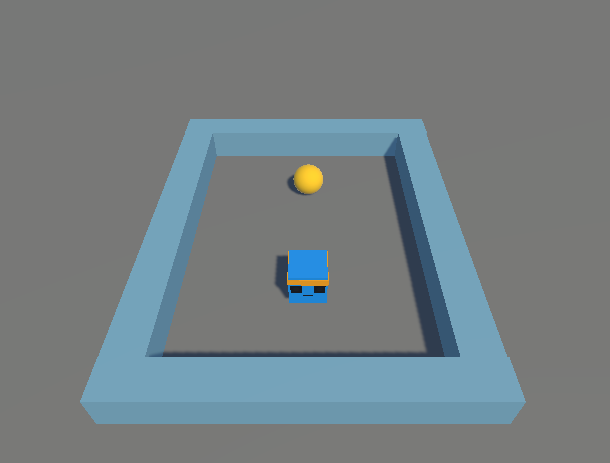
\includegraphics[width=0.5\textwidth]{Images/MoveToGoal.png}
\end{center}
\caption{Move to goal scene}
\label{pic8}
\end{figure}

The first thing we need to do is create an agent script component, which would inherit from the class \texttt{Agent}. Our class would only have to know the position of the goal (it would be a Serialized Field), from the parent class we would need to override the following methods:
\begin{itemize}
    \item \texttt{OnEpisodeBegin} - Every time an episode finished this method is called, so the positions of the goal and agent should be reset. Note: If we reset to the same position every time, the model will become over fitted only go to its learnt position (even if we move the goal). In order to avoid this, it should reset to a random position.
    \item \texttt{CollectObservations} - this method takes a sensor parameter with the class \texttt{VectorSensor}, here the positions of our agent and goal should be added.
    \item \texttt{OnActionReceived} - its plan to take continuous numeric data for the movement of the x axis and z axis, so in this method through the parameter with the class \texttt{ActionBuffers} we can take the before mentioned data and move our agent.
    \item \texttt{Heuristic} - this method works only if the agent's behaviour is set to Heurstic only mode and in our case, its used to test the environment if it works properly.
\end{itemize}

Now we can add the script component to our game object and it should look something like this:
\begin{figure}[h]
\begin{center}
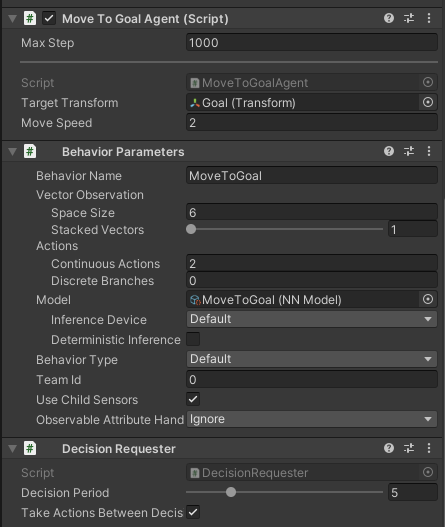
\includegraphics[width=0.35\textwidth]{Images/movetogoalcomponent.png}
\end{center}
\caption{Move to goal agent component}
\label{pic9}
\end{figure}

To optimize learning, the environment should be put in a prefab and instantiated in a the scene multiple times for better results while learning. When done learning, we can use only one environment.

Now, we should determine when the episode ends and the agent gets a positive reward: when it touches the goal. 
And, the episode ends and the agents gets a negative reward: when it touches the walls.

From the figure \ref{pic9}, the first noticeable thing is the max step. This has to be environment specific so that the episode resets and that the agent is not motivated to just stay in one place for the best reward. Next this is that the Continuous Actions are set to two as that's how we move our agent (in the two axes). Also we had to add a decision requester and that's nearly it.

The final thing is that we need to execute the commands to train our agent.  The command is \texttt{mlagents-learn MoveToGoal.yaml --run-id=MoveToGoal}. For this example, the configuration file doesn't really matter. Note: we can use the command \texttt{tensorboard --logdir} to see how our model is progressing in our environment (see figure \ref{pic10}).

\begin{figure}[ht]
\begin{center}
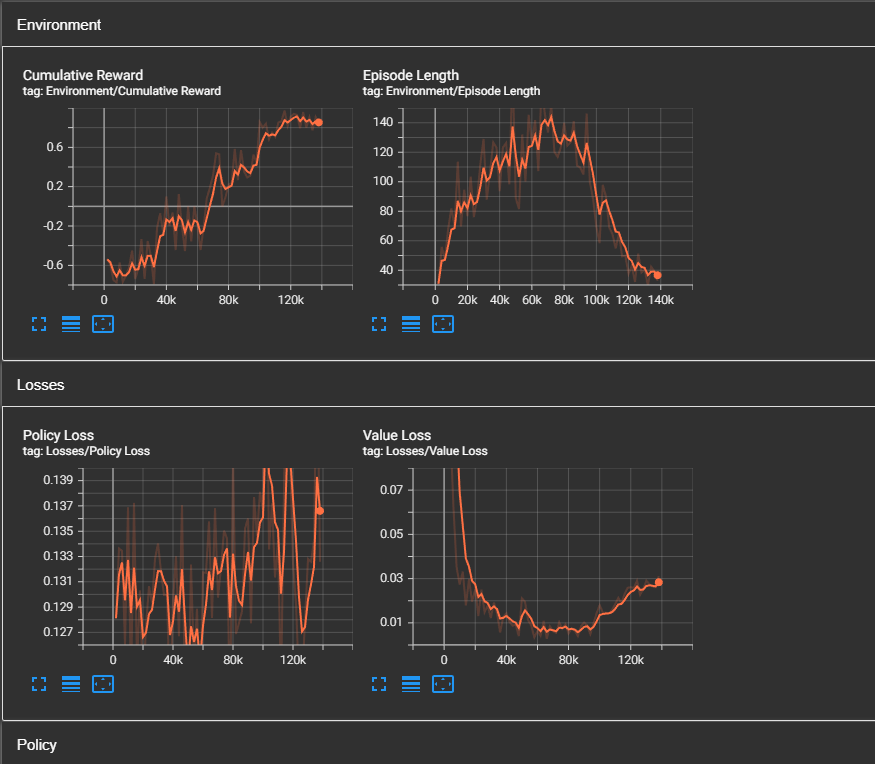
\includegraphics[width=0.4\textwidth]{Images/tensorboard.png}
\end{center}
\caption{Tensorboard of MoveToGoal example}
\label{pic10}
\end{figure}

When we see good progress, we can go ahead and stop the learning. The model will be saved in a \texttt{.onnx} (Open Neural Network Exchange Format) file which we can use for a brain (model) later. And that's basically it, we successfully trained our first NN model, we can use that brain for whatever purpose we want.

\subsection{Dungeon escape}

I want to showcase the next example for the power of ML-Agents and what it is capable of. This game is one of the many ML-Agents \cite{MLAgents} examples, it is a simple game where the players need to escape the dungeon by taking the key and unlocking the door, while being guarded by a dragon.

\begin{figure}[h]
\begin{center}
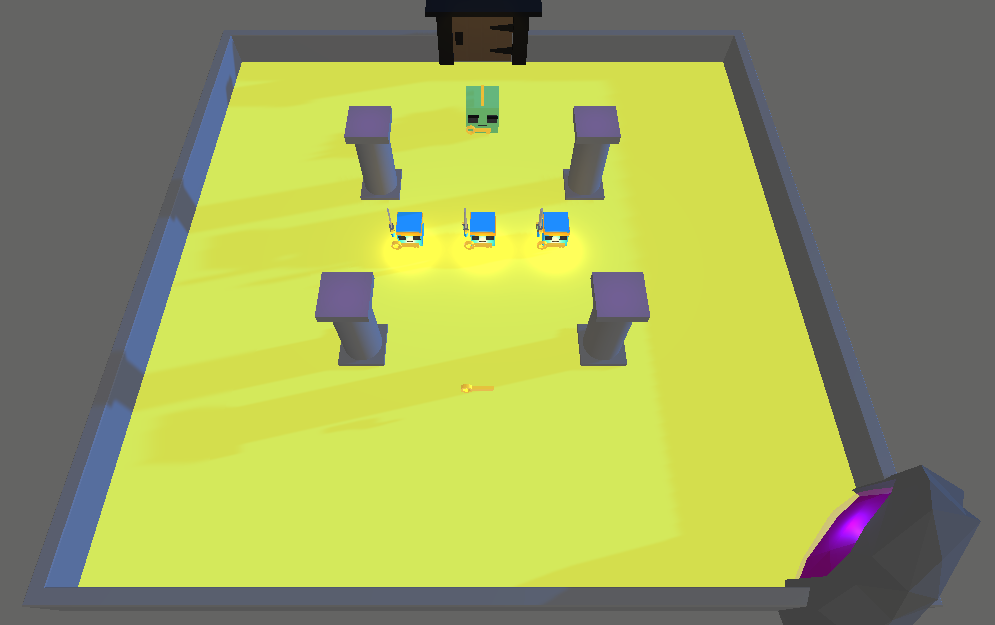
\includegraphics[width=0.5\textwidth]{Images/DungeonEscape.png}
\end{center}
\caption{Dungeon escape example}
\label{pic11}
\end{figure}

What is interesting for this example is that the agent has a ray perception sensor in 3D and its observations are visual, rather than numeric.

\begin{figure}[h]
\begin{center}
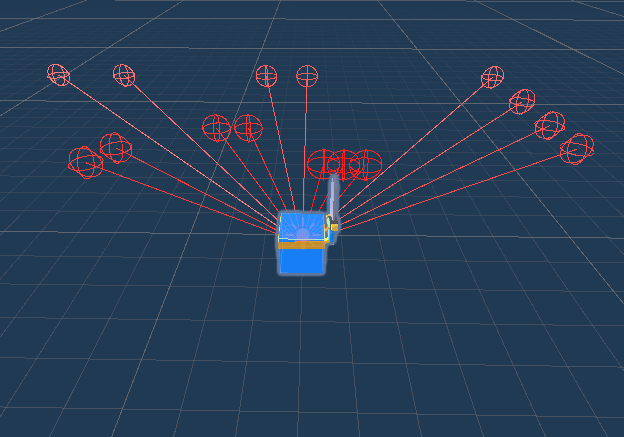
\includegraphics[width=0.3\textwidth]{Images/AgentDungeonEscape.png}
\end{center}
\caption{Ray perception sensor on an agent}
\label{pic12}
\end{figure}

This examples takes use of the \texttt{SimpleMultiAgentGroup} and the agents register to it (the agents are our knights in the figure \ref{pic11}). The agents take 6 discrete actions, two for rotation and four for direction movement. They can pick up a key and if they have it they can unlock the door and get a reward. Or if an agent collides with the dragon, both the dragon and the agent die.

\subsection{Pyramids}

\chapter{Conclusion}
\label{ch4}

It can be easily said that the current and past games rely on the more simple and stable techniques. It is because of that development that players are growing weary of deterministic and plain AI in games. So, as it is a race for better game graphics, now I think there exists a race for a more in-depth game AI with NNs, BTs, fuzzy logic, genetics algorithms etc. 

I think the future takes us step by step towards virtual autonomous characters that are lifelike, intelligent and convey empathy and I only think it is a matter of time before we can reach that. I know that till now I was showcasing techniques that sell the intelligence and not real AI. But, also I know that there is a definite progress in the techniques shown. With creating a well thought out game architecture/system and combining it with new AI techniques, I think that the impossible can become possible.

True AI is far from complete, unpredictable

\cleardoublepage
\addcontentsline{toc}{chapter}{Literature}
\bibliography{literature}
\bibliographystyle{plainnat}

\end{document}